
\documentclass[ms.tex]{subfiles}
\begin{document}

\section{Application to Observations}
\label{sec:h3}

\begin{figure*}
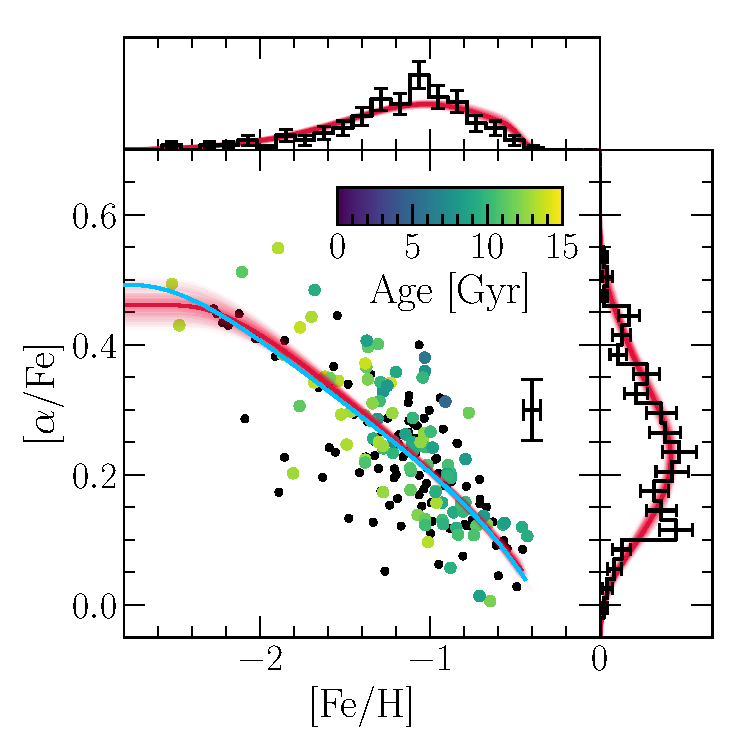
\includegraphics[scale = 0.5]{gsefit_afe_feh.pdf}
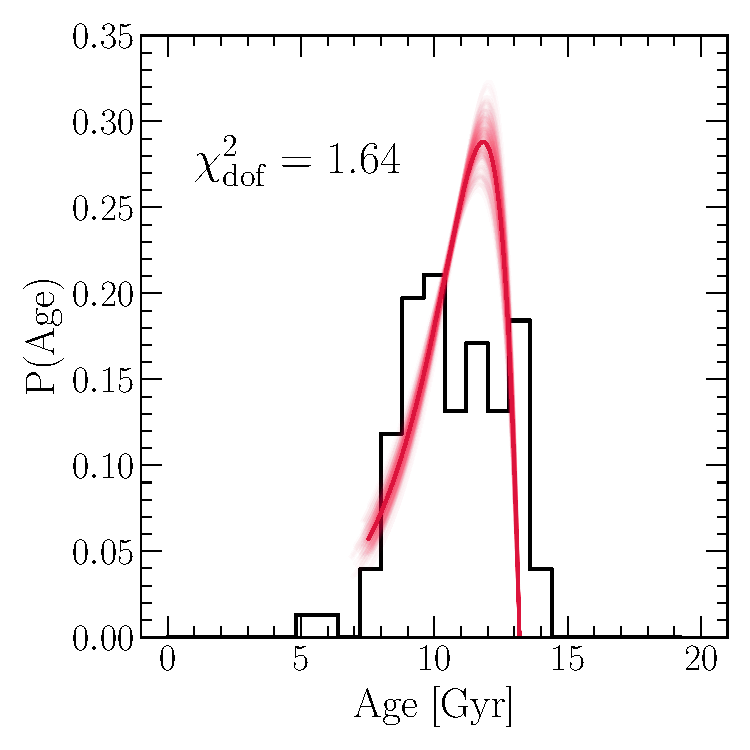
\includegraphics[scale = 0.42]{gsefit_agedist.pdf}
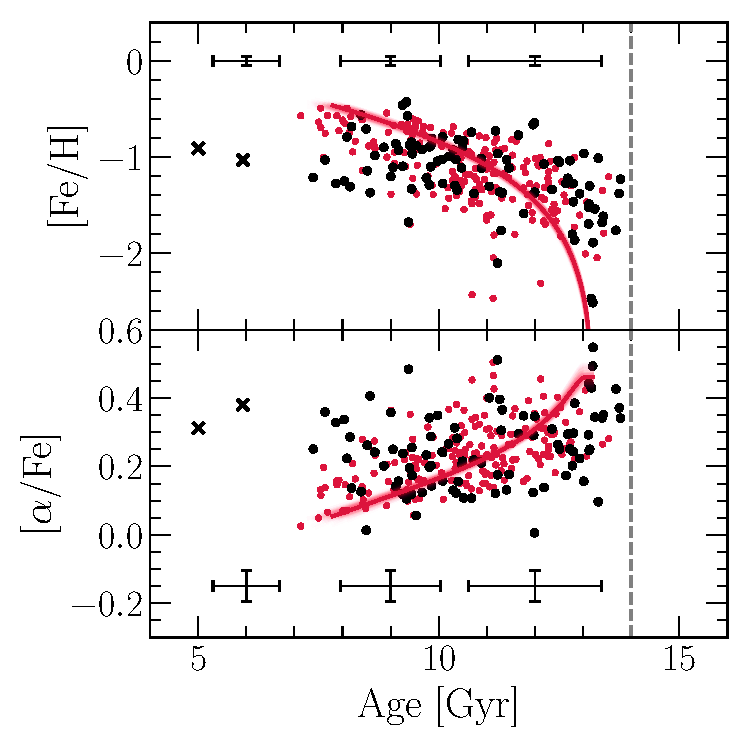
\includegraphics[scale = 0.42]{gsefit_amr.pdf}
\caption{
\textbf{Left}: Our GSE sample in the~\afe-\feh~plane and the associated
marginalized distributions.
Stars are colour-coded according to their age where available and are otherwise
plotted in black.
The best-fit chemical evolution track and distributions in~\afe~and~\feh~are
shown as solid red lines.
The median~\feh~and~\afe~errors of the sample are shown by the error bar to the
right of the data. 
\textbf{Middle}: The age distribution measured for our GSE sample (black) and
the best-fit age distribution based on the SFH of our model (red, solid).
We additionally plot the age distribution obtained when we convolve the best-fit
distribution with an uncertainty of~$\sigma(\log_{10}(\text{age}))$ including
the prior that age~$<$ 14 Gyr as in the H3 age measurements.
\textbf{Right}: The age-\feh~and age-\afe~relations of our GSE sample (black)
and our best-fit chemical evolution model (red).
The median~\feh,~\afe, and age uncertainties are shown by the error bars to the
left of the data in each panel.
We plot the two stars that we exclude from our fit as our black X's (see
discussion in~\S~\ref{sec:h3:gse}).
In all panels, we subsample 200 sets of parameter choices~$\{\theta\}$ from our
likelihood distribution (see Fig.~\ref{fig:gse_corner}) and plot their
predictions as high transparency lines to provide a sense of the fit precision
in the observed space.
}
\label{fig:gse_bestfit}
\end{figure*}

\begin{itemize}

	\item Next we apply our fitting method to two dwarf satellite remnants
	observed in the Milky Way halo by the H3 survey~\citep[survey design:
	][]{Conroy2019}.
	The first is a relatively well-studied system: the Gaia-Sausage Enceladus
	\citep[GSE;][]{Belokurov2018, Helmi2018}, believed to be responsible for
	a major merger event early in the Milky Way's history~\citep{Chaplin2020}
	which contributed~$10^9 - 10^{10} \msun$ of total stellar mass
	\citep{Deason2019, Fattahi2019, Mackereth2019, Vincenzo2019}, including
	eight globular clusters in the stellar halo~\citep{Myeong2018}.
	The second is a less well-studied system: the Wukong stellar stream,
	a prograde structure chemically distinct from the GSE which sits between it
	and the Helmi Streams~\citep{Helmi1999} in energy--angular momentum
	space~\citep{Naidu2020, Naidu2022}.
	We provide an overview of the H3 survey below and discuss our GCE model
	fits to the GSE and Wukong progenitors in~\S\S~\ref{sec:h3:gse}
	and~\ref{sec:h3:wukong} below.

\end{itemize}

\subsection{The H3 Survey}
\label{sec:h3:survey}

The H3 survey~\citep{Conroy2019} is collecting medium-resolution spectra of
$\sim$300,000 stars in high-latitude fields ($\left|b\right| > 20^\circ$).
Spectra are collected from the Hectochelle instrument on the MMT
\citep{Szentgyorgyi2011} which delivers~$R \approx 32,000$ spectra over the
wavelength range of~$5150 - 5300$~\AA.
Spectral lines in this wavelength range are dominated by iron-peak elements,
but it does safely include the FeI/MgI blended line at 5167~\AA~as well as the
strong MgI lines at 5173 and 5184~\AA~(see Fig. 6 of~\citealp{Conroy2019}).
Throughout this section, the alpha element abundances we refer to are therefore
Mg abundances specifically, whereas in previous sections an alpha element
refers to any species where the only statistically significant enrichment
source is a metallicity-independent yield from massive stars.
\par
The survey selection function is deliberately simple: the primary sample
consists of stars with~$r$ band magnitudes of~$15 < r < 18$ and Gaia parallaxes
$< 0.3$ mas (this threshold has evolved over the course of the survey as the
Gaia astrometry has become more precise).
Stellar parameters are estimated via the~\textsc{MINESweeper} program
\citep{Cargile2020}, which fits grids of isochrones, synthetic spectra and
photometry to the Hectochelle spectrum and broadband photometry from Gaia,
Pan-STARRS, SDSS, 2MASS and WISE with the Gaia parallax used as a prior.
The fitted parameters include radial velocity, spectrophotometric distance,
reddening,~\feh,~\afe~and age.
The default analysis includes a complicated prior on age and distance (see
\citealt{Cargile2020} for details).
We have also re-fit high signal-to-noise data with a flat age prior for cases
where ages play an important role, and in this paper we use the catalog that
assumes this flat prior.

\subsection{The Gaia-Sausage Enceladus}
\label{sec:h3:gse}

\begin{figure*}
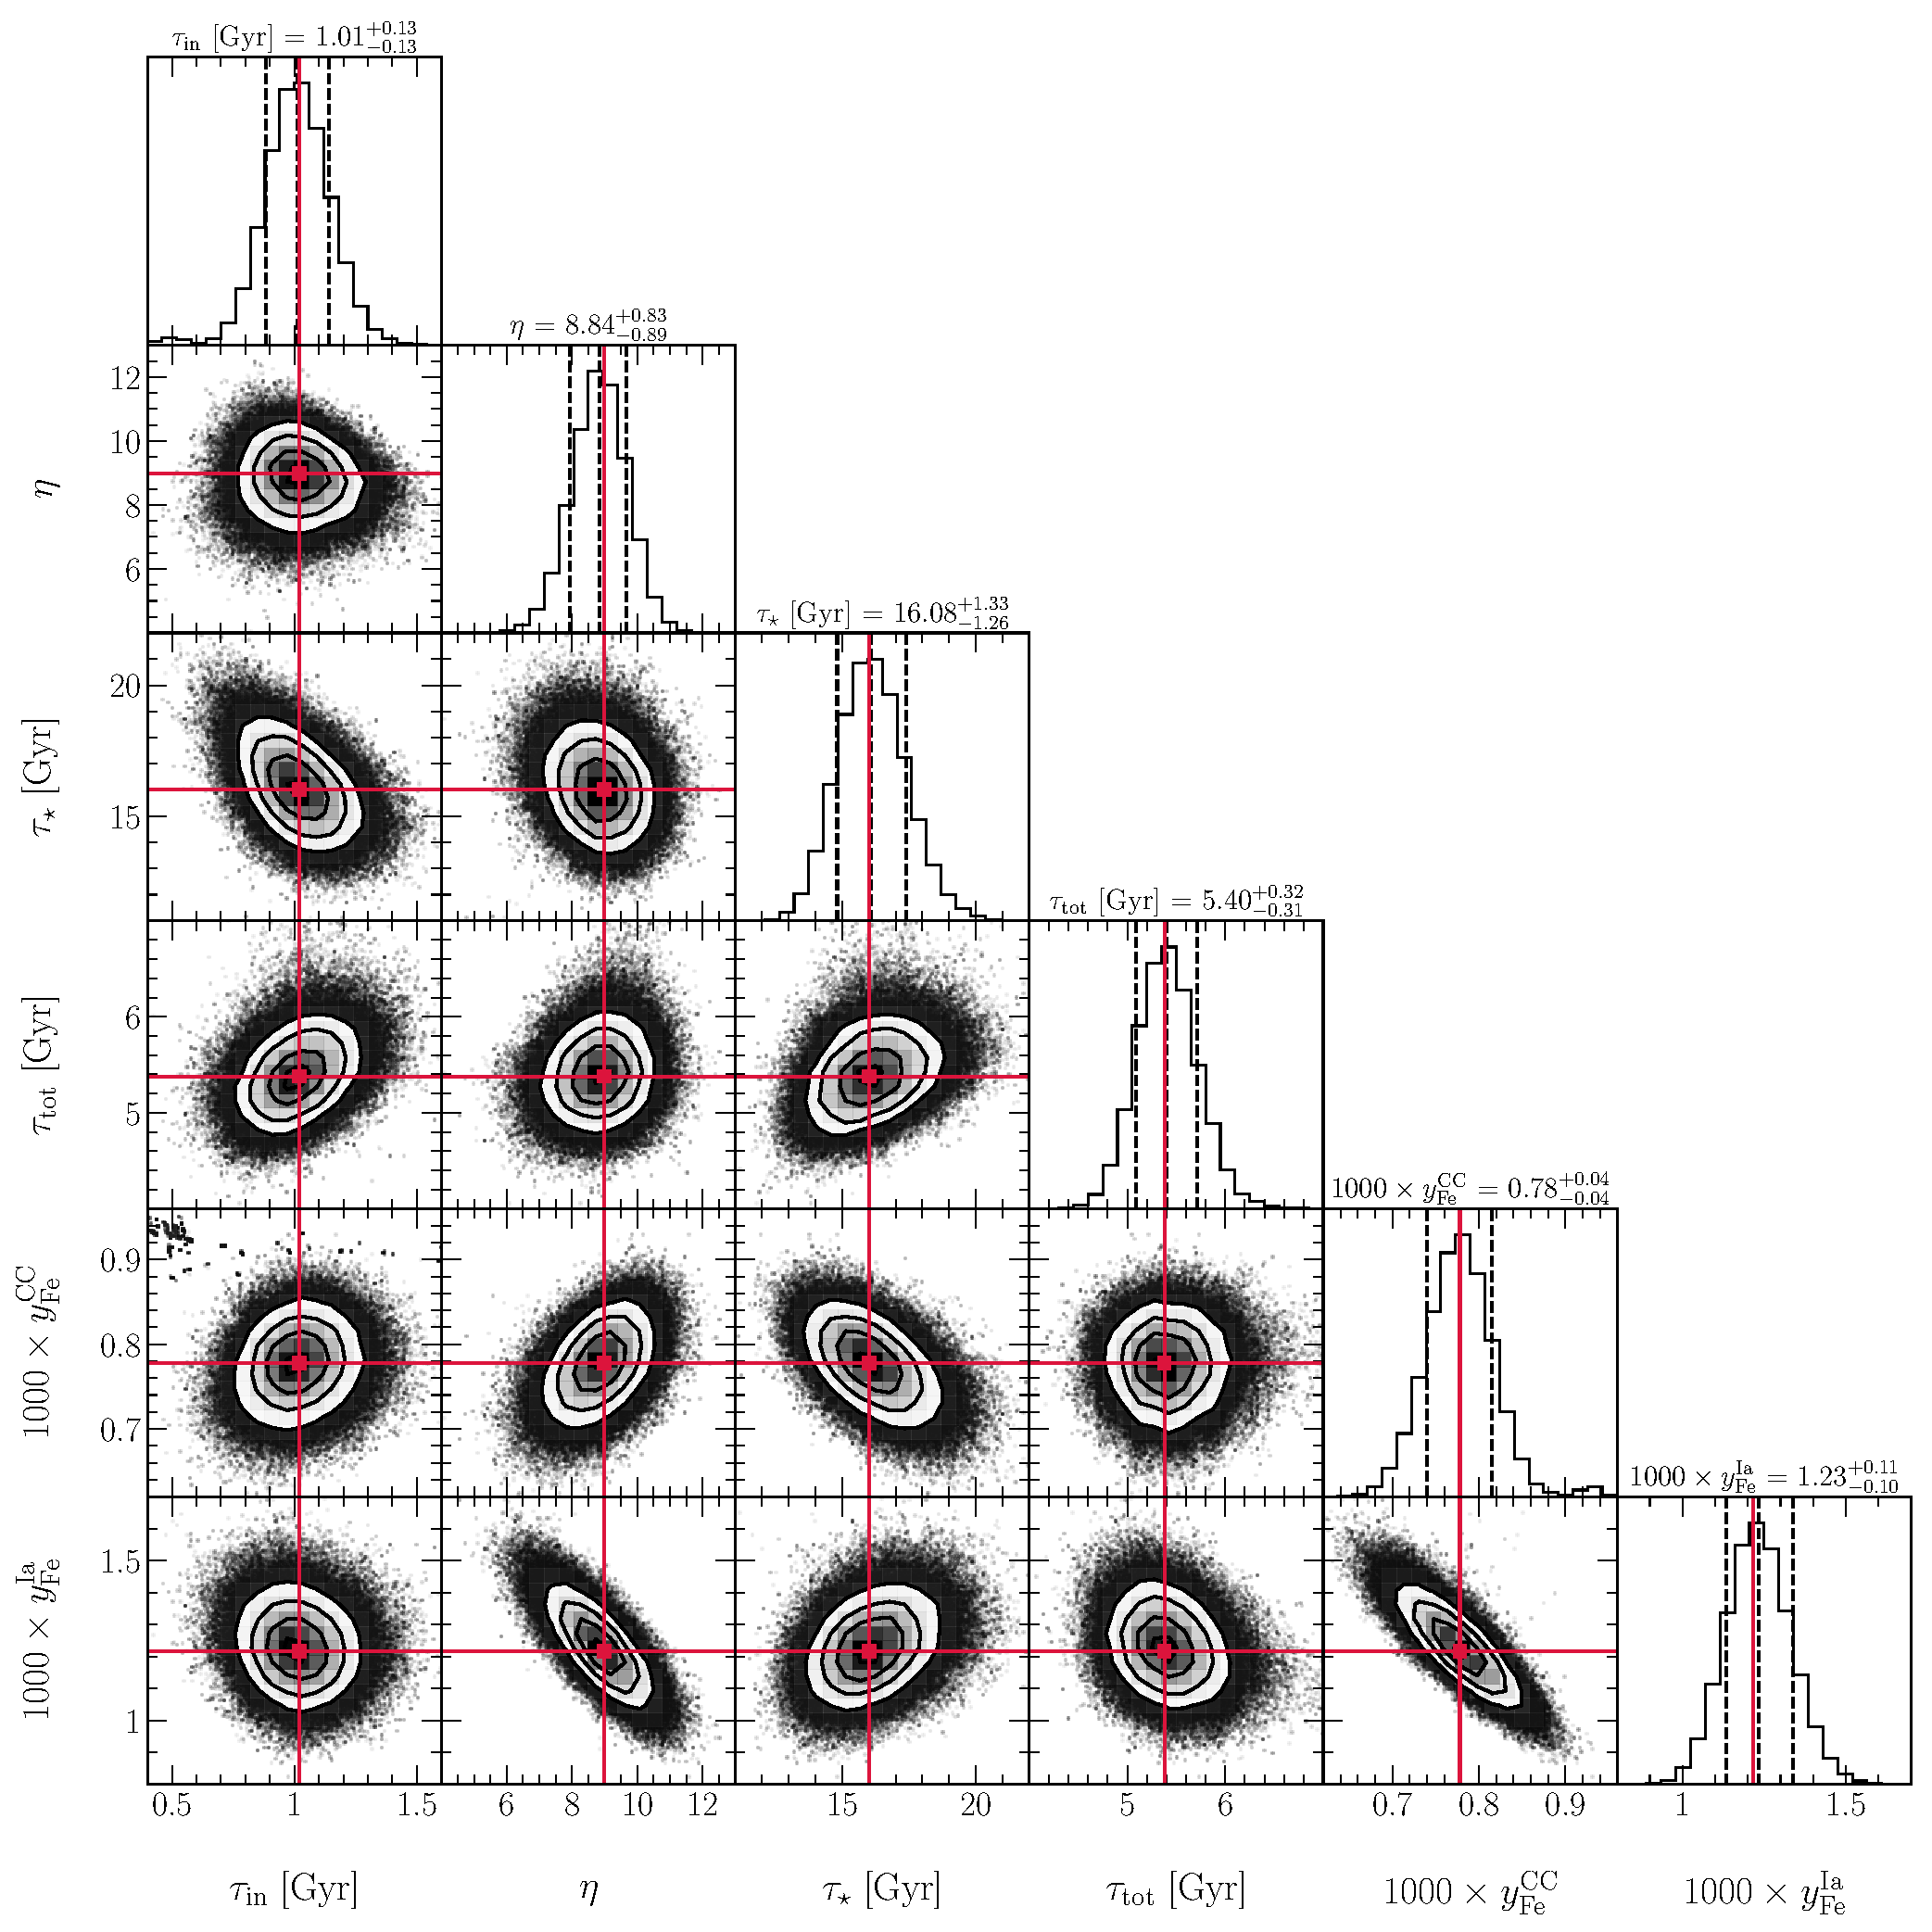
\includegraphics[scale = 0.45]{gsechem_512k.pdf}
\caption{
The ``corner-plot'' showing the results of our fitting method applied to GSE
stars observed by the H3 survey.
We show the marginalized likelihood distributions in each parameter along with
their best-fit values and confidence intervals along the diagonal.
Below the diagonal, we show the 2-dimensional cross-sections of the
6-dimensional likelihood function.
Contrary to Fig.~\ref{fig:corner_fiducial}, red ``cross-hairs'' mark the
element of the Markov chain with the maximum statistical likelihood.
}
\label{fig:gse_corner}
\end{figure*}

\begin{figure}
\centering
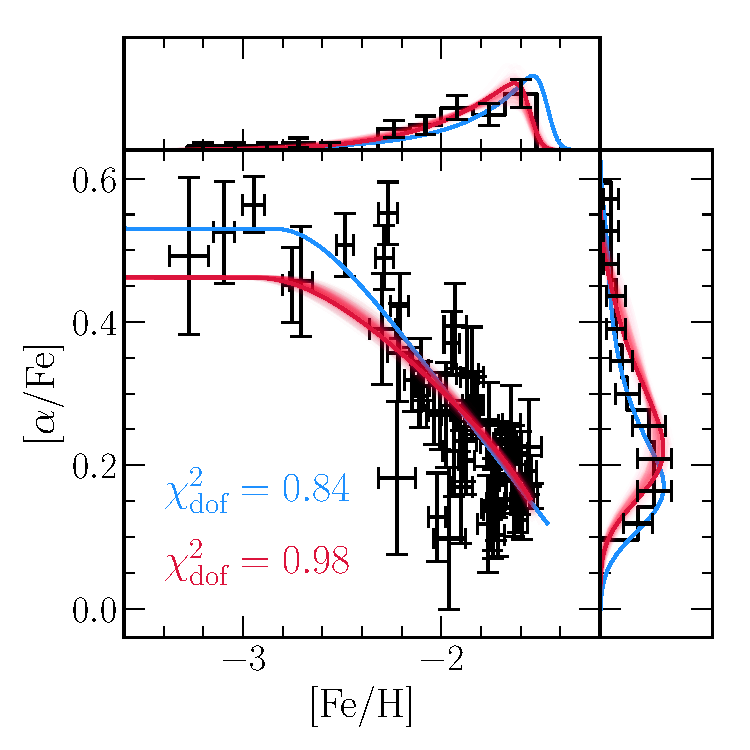
\includegraphics[scale = 0.55]{wukong_bestfit.pdf}
\caption{
Our Wukong sample in the~\afe-\feh~plane and the associated marginalized
distributions.
Error-bars in the central panel denote the measurement uncertainty on
individual stars' abundance measurements, and error-bars in the top and right
panels indicate the uncertainty in the abundance distributions assuming
$\sigma = \sqrt{N}$ from sampling noise.
We plot our best-fit chemical evolution model in red (see discussion
in~\S~\ref{sec:h3:wukong}, with 200 additional sets of parameter choices
subsampled from our likelihood function to give a sense of the fit precision.
}
\label{fig:wukong_bestfit}
\end{figure}

\begin{figure*}
\centering
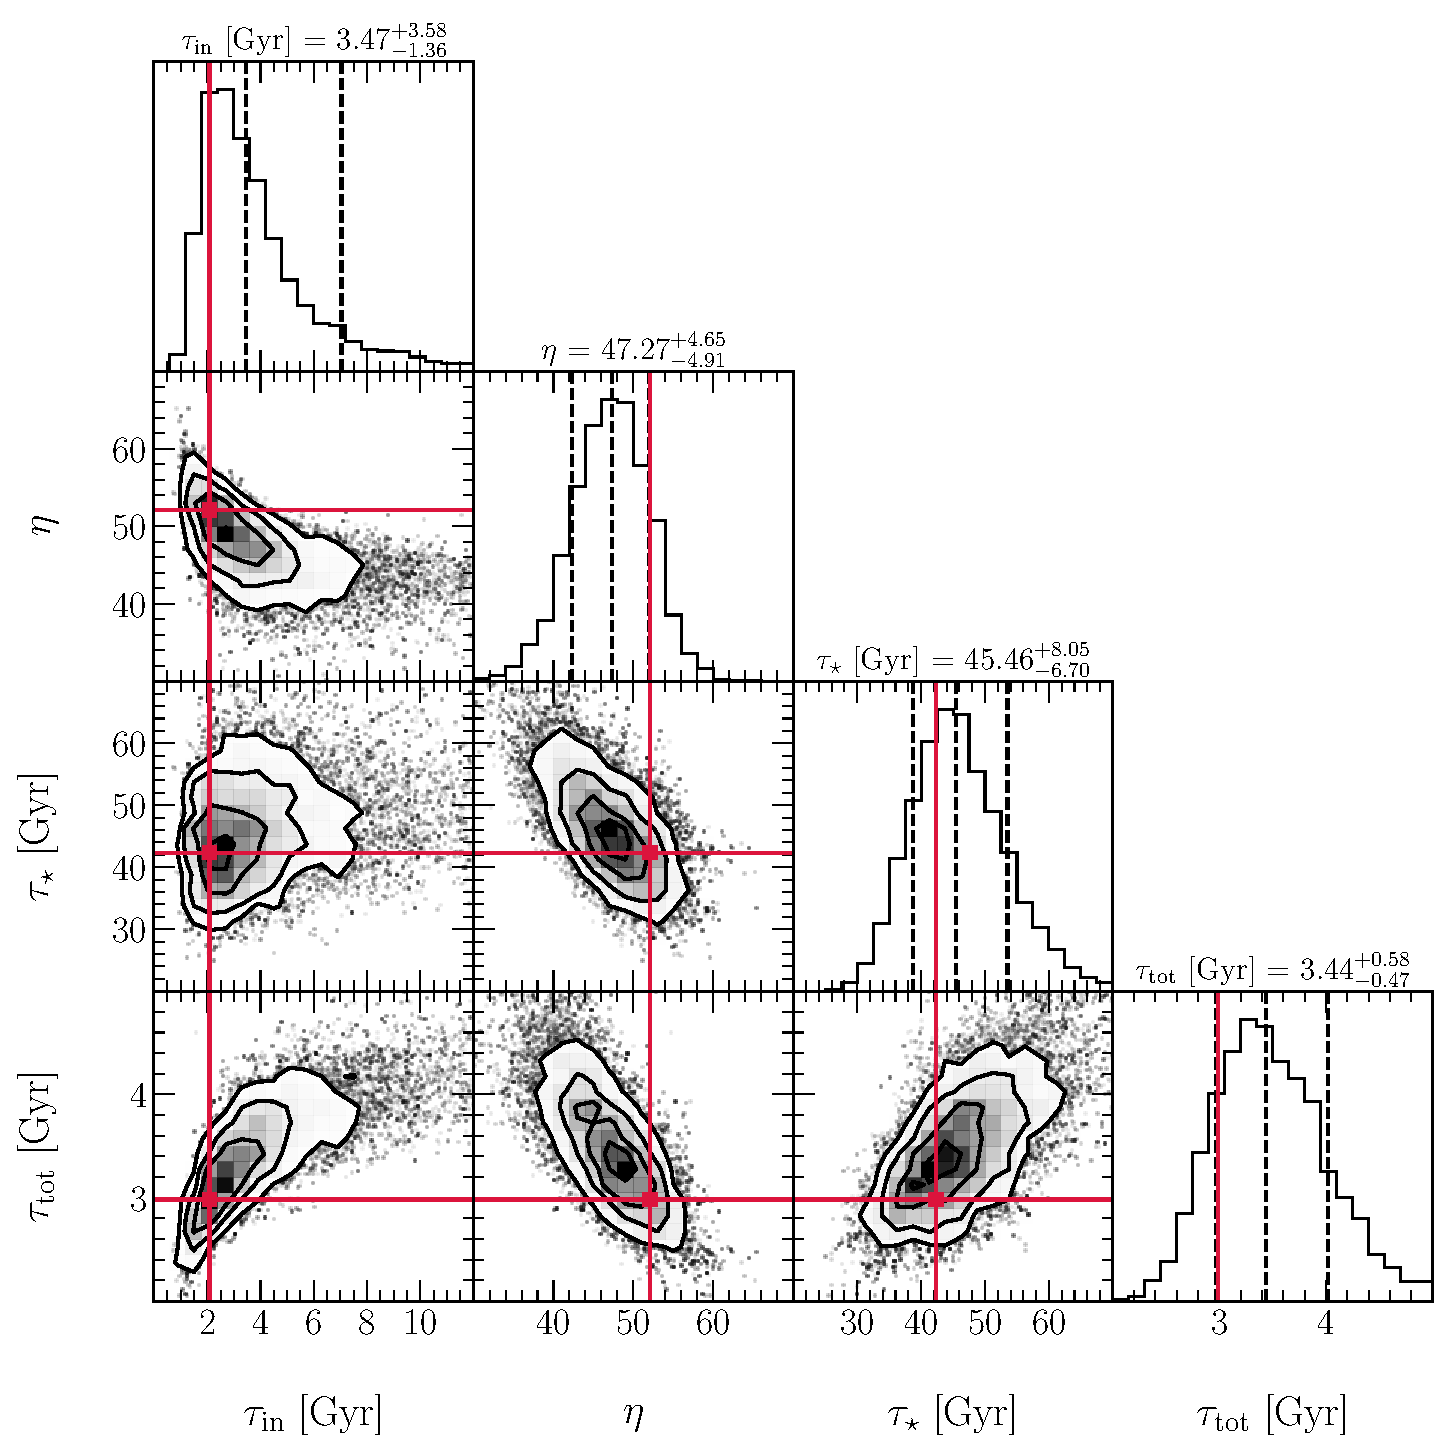
\includegraphics[scale = 0.50]{wukong_expifr_102k4.pdf}
% 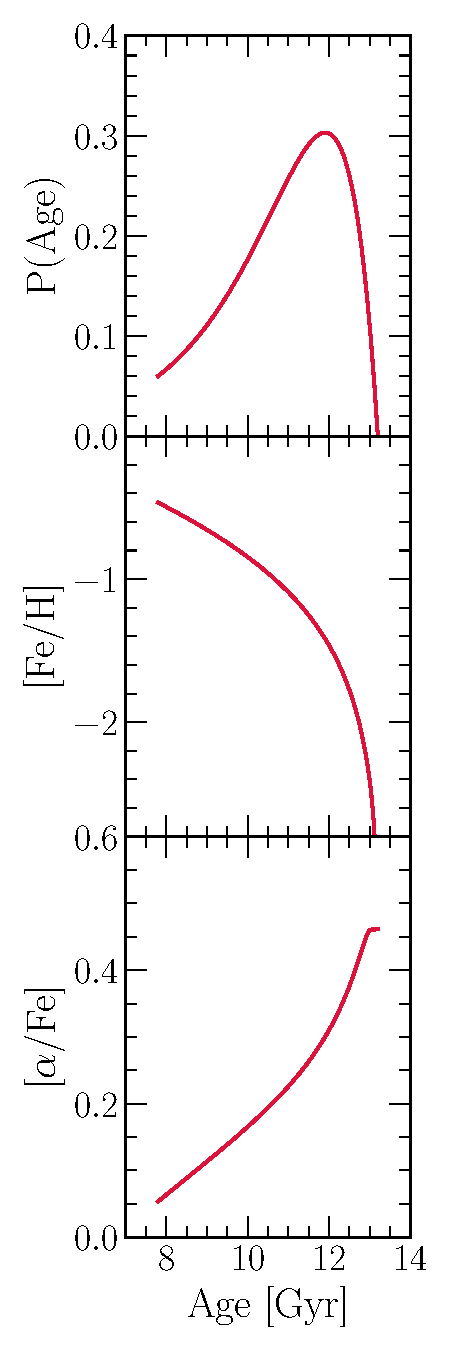
\includegraphics[scale = 0.52]{wukong_agedist_amr.pdf}
\caption{
\textbf{Left}: The ``corner-plot'' showing the results of our fitting method
applied to the Wukong stream, as in Fig.~\ref{fig:gse_corner}, but with fixed
SN yields.
\textbf{Right}: The predicted age distribution (top), age-\feh~relation
(middle), and age-\afe~relation (bottom).
We subsample 200 parameter choices from our likelihood distribution in the
left hand panels and plot the resultant predictions as high-transparency lines
to give a sense of the fit precision.
}
\label{fig:wukong_corner}
\end{figure*}

\begin{figure*}
\centering
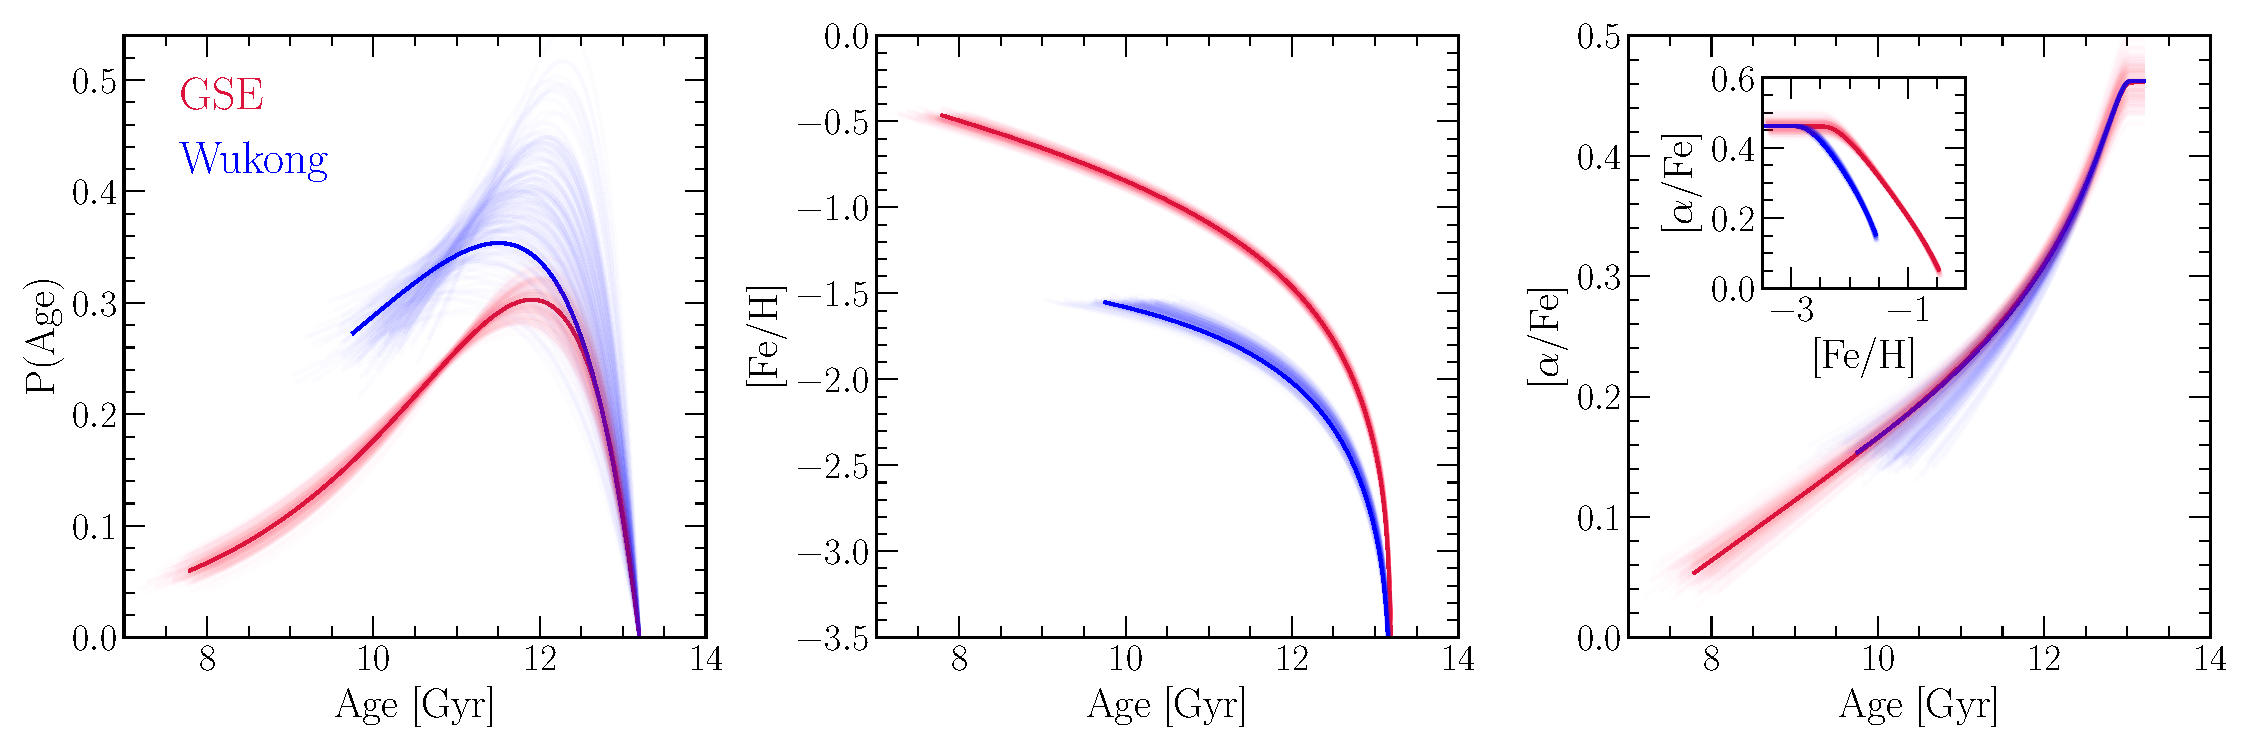
\includegraphics[scale = 0.50]{gse_wukong_comparison.pdf}
\caption{
Comparison between GSE and Wukong best-fits.
}
\label{fig:gse_wukong_comp}
\end{figure*}

\begin{itemize}

	\item Our sample from the GSE consists of 189 stars, 95 of which have
	age measurements.
	These stars span metallicities of~$\feh \approx -2.5$ to~$-0.4$ and
	$\afe \approx 0$ to $+0.55$.
	Abundance uncertainties range from~$\sim$0.02 to~$\sim$0.12 in
	both~\feh~and~\afe~with median values near~$\sim$0.05.
	Of the stars with age measurements, the youngest is~$\sim$5 Gyr old and the
	oldest is~$\sim$13.8 Gyr old.
	All inferred ages, however, incorporate a prior imposed by the H3 pipeline
	which requires all values to be below 14 Gyr, preventing the log-normal
	nature of age uncertainties from populating the~$\sim14 - 20$ Gyr range.
	Every age measurement has a statistical uncertainty below
	$\sigma(\log_{10}(\text{age})) = 0.05$, corresponding to a measurement
	precision of~$\lesssim$12\%.
	Due to the difficulty associated with measuring stellar ages both
	accurately and precisely~\citep{Soderblom2010, Chaplin2013}, we adopt this
	value of~$\sigma(\log_{10}(\text{age})) = 0.05$ as the minimum uncertainty
	to account for any systematic errors that may be present.
	This consequently applies to the whole subset of our sample that has age
	measurements.
	Because H3 selects targets based only on a magnitude range and a maximum
	parallax, the selection function in chemical space should be nearly
	uniform (i.e.~$\script{S}(\script{M}_j | \{\theta\}) \approx 1$ for all
	points along the evolutionary track~$\script{M}_j$).
	We therefore take the weights appearing in our likelihood function to be
	proportional to the SFH alone (equations~\ref{eq:likelihood}
	and~\ref{eq:weights}; see discussion in~\S~\ref{sec:fitting}).

	\item The left panel of Fig.~\ref{fig:gse_bestfit} shows our sample in
	the~\afe-\feh~plane along with the associated marginalized distributions.
	The mode of the MDF is near~$\feh = -1$ and~$\afe = +0.25$, and the
	``knee'' associated with the onset of SN Ia enrichment is apparent
	near~$\feh \approx -2$, though there are only a few stars in our sample
	in this region of chemical space.
	Invoking the equilibrium arguments of~\citet{Weinberg2017}, the knee
	occurring at low metallicity and an MDF dominated by low metallicity stars
	is indicative, respectively, of slow star formation (i.e. high~$\tau_\star$)
	and a low equilibrium abundance due to strong outflows (i.e. high~$\eta$).
	This is expected for a dwarf galaxy progenitor where star formation is
	typically slow~\citep[e.g.][]{Hudson2015} and the gravitational potential
	well is shallow due to low stellar and halo masses.
	Furthermore, the alpha-enhanced nature of the MDF is indicative of an SFH
	which was truncated early in the GSE's history before SN Ia enrichment
	could produce enough Fe to reach solar~\afe, a result which also expected
	given that the age distribution, shown in the middle panel, is dominated
	by old stars ($\gtrsim 8$ Gyr).
	The truncation of the age distribution likely reflects the quenching of
	star formation in the GSE progenitor as a consequence of ram pressure
	stripping by the hot halo of the Milky Way after its first infall~$\sim$10
	Gyr ago~\citep{Bonaca2020}.
	The age-metallicity relation (AMR) (both age-\feh~and age-\afe) has a
	considerable amount of scatter, in large part because of the considerable
	age uncertainties.

	\item We note the presence of two outliers at ages of~$\sim$5 and 6 Gyr,
	marked by X's in the right panel.
	These stars have abundances typical of the rest of the GSE population but
	are anomalously young.
	It's likely that these are blue stragglers: stars which are thought to be
	made hotter and more luminous by accretion from a binary companion.
	As a result, they occupy a region of the CMD which is normally occupied by
	much younger, more massive stars, biasing their age measurements to low
	values~\citep[e.g.][]{Bond1971, Stryker1993}.
	We therefore omit these stars from our chemical evolution model fit to the
	GSE, including only those which are older than~$\sim$7 Gyr.

	\item The steadily sloped decline of~\afe~with increasing~\feh~and the
	approximately monotonic nature of the age-\feh~and age-\afe~relations
	incidicate a smooth SFH.
	If the GSE had experienced a burst in star formation at some point in its
	history, this would be accompanied by a sudden increase in~\afe~followed by
	a decline back toward the pre-burst value due to the temporarily perturbed
	ratio of CCSN and SN Ia rates~\citep{Johnson2020}.
	We therefore fit the GSE with a smooth evolutionary model, adopting the
	same exponential infall history as our mock samples described
	in~\S~\ref{sec:mocks:fiducial}.

	\item Fig.~\ref{fig:gse_corner} shows the likelihood distribution we obtain
	for the GSE by applying our fitting method.
	We indeed find that the best-fit evolutionary model implies slow star
	formation ($\tau_\star \approx 16$ Gyr) and strong outflows
	($\eta \approx 9$), qualitatively similar to our mock samples.
	Our fit additionally suggests that the Fe yields are
	$\yfecc = \scinote{7.78^{+0.37}_{-0.38}}{-4}$ and
	$\yfeia = \scinote{1.23^{+0.11}_{-0.10}}{-3}$ on the scale where the alpha
	element yield is fixed at~$\yacc = 0.01$.
	With these Fe yields, our fit to the GSE data suggests that CCSNe account
	for~$\yfecc / (\yfecc + \yfeia) \approx$ 40\% of the Fe in the universe.
	This value may however be influenced by the H3 pipeline which enforces a
	prior that~$\afe \leq +0.6$~\citep{Cargile2020} - if the~\afe~``plateau''
	in nature occurs occurs near this value, it could be significantly biased
	to lower values.

	\item As discussed in~\S~\ref{sec:onezone} and quantified in Appendix
	\ref{sec:yield_outflow_degeneracy}, these yields are subject to the
	yield-outflow degeneracy along with~$\eta$ and~$\tau_\star$, and our
	adopted value of~$\yacc = 0.01$ is only intended to set some overall scale
	to these values which can be adjusted as necessary.
	Consequently, only relative rather than absolute values carry any meaning.
	In the absence of winds (i.e.~$\eta = 0$) but with otherwise the same
	evolutionary parameters, the MDF is predicted to have a peak
	near~$\feh \approx -0.5$ with a tail toward low metallicities and a
	sharp cutoff at higher metallicities, indicating that star formation in the
	GSE was slow enough that it would have only achieved~$\sim$one-third solar
	metallicity within 5.4 Gyr of star formation even with the largest sink
	term in the enrichment rates removed.
	If star formation instead sped up to~$\tau_\star = 1$ Gyr, corresponding
	approximately to the expected value if the GSE were composed entirely of
	molecular hydrogen while forming stars at~$z \gtrsim 1$~\citep{Tacconi2018},
	then the predicted MDF is still peaked near~$\feh \approx -1$ but is more
	symmetric and less skewed toward lower~\feh~as in the GSE data (see
	Fig.~\ref{fig:gse_bestfit}).
	In order to predict an MDF dominated by solar metallicity stars, this model
	requires~\textit{both} weaker outflows and more efficient star formation.

	\item The infall timescale~$\tau_\text{in}$ and the total duration of
	star formation~$\tau_\text{tot}$, however, are orthogonal to the
	yield-outflow degeneracy (see Appendix~\ref{sec:yield_outflow_degeneracy}),
	indicating that these absolute values do carry meaning.
	The infall history is sharp ($\tau_\text{in} \approx 1$ Gyr), as expected
	given the alpha-enhanced mode of the MDF.
	Star formation lasted~$5.40^{+0.32}_{-0.31}$ Gyr after an onset assumed to
	occur at a lookback time of 13.2 Gyr based on the~\textsc{UniverseMachine}
	semi-analytic model~\citep[][see discussion
	in~\S~\ref{sec:mocks:fiducial}]{Behroozi2019}.
	This corresponds to the GSE's last episode of star formation occurring
	$7.80^{+0.31}_{-0.32}$ Gyr ago, consistent with the age distribution shown
	in Fig.~\ref{fig:gse_bestfit}.

	\item We plot the predictions of our best-fit model over the GSE data in
	Fig.~\ref{fig:gse_bestfit}, along with 200 additional parameter choices
	selected from the Markov chain plotted as high transparency lines to
	provide a visual sense of the fit uncertainty.
	We convolve the~\feh~and~\afe~distributions with a gaussian whose width
	is the median measurement uncertainty in each quantity; we do the same for
	the ages with a log-normal distribution.
	Overall, this model is a reasonable description of the data.
	In detail, the model predicts a slightly broader~\feh~distribution and
	slightly more peaked age distribution than the data.
	We quantify the quality of the fit in the same manner described in the
	final paragraph of~\S~\ref{sec:mocks:fiducial_fit}, finding
	$\chi_\text{dof}^2 = 1.34$.
	As a consequence of the considerable measurement uncertainties in stellar
	ages, it might appear at first glance that the model is a poor fit to the
	age-\feh~and age-\afe~relation.
	To demonstrate this, we subsample 95 stars (the same number of stars from
	our GSE sample that have age measurements) from our best-fit SFH and
	perturb their ages and abundances by the corresponding median uncertainties
	of the sample and plot the results in the right panel of
	Fig.~\ref{fig:gse_bestfit} for comparison.
	The resultant samples occupies a similar region of the age-\feh~and
	age-\afe~planes as the data, indicating that the model is indeed a good
	description of these data.
	We do however note an additional~$\sim6$ or~$7$ potential blue stragglers
	with ages of~$\sim8 - 9$ Gyr,~$\feh \approx -1.2$, and~$\afe \approx +0.4$.
	These stars are less obviously blue stragglers than the two at ages of 5
	of 6 Gyr and would not have stuck out as outliers if we did not have the
	GCE model to compare to.
	If we were to remove these stars from our sample, our model would be an
	even better description of the GSE by lowering the height of the age
	distribution at~$\sim8 - 9$ Gyr.

	\item In~\S~\ref{sec:mocks}, we found that our model accurately
	recovered the known evolutionary timescales of mock samples, including the
	total duration of star formation and the e-folding timescale of the infall
	history.
	However, we fit our mock samples with the exact underlying GCE model and
	same numerical code from which they were generated, placing the exact same
	systematic effects in the data as in the model.
	In practice, the systematics affecting the data and the model are generally
	different, and the evolutionary history built into the model is not
	necessarily a perfect description of the galaxy.
	To demonstrate this, we conduct an additional fit to our GSE sample and
	leave out the age information.
	The SN yields and mass-loading factor inferred in this case are
	consistent with our original fit, but in comparison it significantly
	overestimates the infall timescale 
	$\tau_\text{in} = 2.18^{+0.43}_{-0.56}$), the SFE timescale
	($\tau_\star = 26.60^{+4.83}_{-6.11}$) and the duration of star formation
	($\tau_\text{tot} = 10.73^{+1.76}_{-2.69}$).
	We show the evolutionary track in chemical space and age distribution
	predicted by this model in Fig.~\ref{fig:gse_bestfit}.
	Without any age information, our method achieves an accurate description of
	the abundance distributions, but the predicted age distribution is
	significantly more extended than the data.
	Although our results presented in~\S~\ref{sec:mocks} suggest that it
	is theoretically possible to infer GCE model parameters from detailed
	abundances without any age measurements, this comparison suggests that this
	information is much more important in practice for pinning down
	evolutionary timescales.
	While the most powerful way to provide this information for the likelihood
	function is with individual age measurements, in principle this can also
	be done by, e.g., constructing a prior based on a CMD-derived SFH as in
	\citet{Dolphin2002} and~\citet{Weisz2014b}.

\end{itemize}

\subsection{The Wukong Stream}
\label{sec:h3:wukong}

\begin{itemize}

	\item Our sample from the Wukong stream consists of 57 stars, none of which
	have age information because they are distant red giant stars.
	This sample spans two orders of magnitude in metallicity,
	from~$\feh \approx -3.5$ to~$\sim$-2.5.
	Our GSE stars, however, have reached solar~\afe~while the least alpha-rich
	Wukong star has~$\afe \approx +0.1$.
	Abundance uncertainties range from~$\sim$0.02 to~$\sim$0.10 in
	both~\afe~and~\feh~with median values near~$\sim$0.045.

	\item Fig.~\ref{fig:wukong_bestfit} illustrates our sample the~\afe-\feh~
	plane along with the associated marginalized distributions.
	There are a notable number of stars near the ``knee'' associated with the
	onset of SN Ia enrichment around~$\feh \approx -3$.
	Similar to the GSE but to an even greater extent, the metal-poor and
	alpha-rich nature of the MDF is indicative of slow star formation and
	strong outflows, and the lack of discontinuities in the~\afe-\feh~trend
	indicates a smooth SFH devoid of any starburst events.
	We therefore fit our Wukong sample with the same evolutionary history that
	we modelled both the GSE and our mock samples with, retaining the
	assumption that the H3 selection function is uniform in chemical space (see
	discussion in~\S~\ref{sec:h3:gse}).
	However, because SN yields should be set by stellar physics, we fix their
	values at~$\yfecc = \scinote{7.78}{-4}$ and~$\yfeia = \scinote{1.23}{-3}$
	as determined by our fit to the GSE data.

	% \item The lack of discontinuities in the~\afe-\feh~trend, also as in the
	% GSE, is indicative of a smooth SFH devoid of any starburst events.
	% We therefore fit these data with the same accretion history as in our
	% mock samples and the GSE.
	% However, with our SN yields as free parameters, considerable degeneracies
	% arise in the inferred evolutionary timescales; we saw similar behaviour in
	% our mock sample with no age information (see discussion
	% in~\S~\ref{sec:mocks:variations}).
	% Because SN yields should be set by stellar physics and consequently be the
	% same between the GSE and Wukong, we fix these values
	% at~$\yfecc = \scinote{7.78}{-4}$ and~$\yfeia = \scinote{1.23}{-3}$ as
	% determined by our fit to the GSE data.
	% We retain the assumption that the selection function in chemical space is
	% un-biased (i.s.~$\script{S}(\script{M}_j, \{\theta\}) = 1$ for all points
	% along the evolutionary track~$\script{M}_j$) because H3 is an untargeted
	% survey {\color{red} (right?)}.

	\item The left hand side of Fig.~\ref{fig:wukong_corner} shows the
	``corner-plot'' obtained from fitting this model to our Wukong sample using
	the likelihood function given by equation~\refp{eq:likelihood}.
	The marginalized likelihood distributions are noticably asymmetric, a
	consequence of the degeneracies that arise in the evolutionary timescales
	in the absence of age information.
	We found similar effects in our mock samples with~$f_\text{age} = 0$ and
	in fitting our GSE sample with no age information in~\S~\ref{sec:h3:gse}.
	This fit indicates considerably stronger winds ($\sim5$ times larger
	$\eta$) and slower star formation ($\sim3$ times larger~$\tau_\star$) than
	the GSE.
	Both of these results point to the Wukong progenitor being significantly
	less massive than the GSE progenitor, which is expected since the GSE is
	perhaps the most massive satellite to have merged with the Milky
	Way~\citep{Deason2019, Fattahi2019, Mackereth2019, Vincenzo2019}.
	Our fit additionally indicates that the Wukong progenitor experienced a
	more extended infall history with an accretion timescale of
	$\tau_\text{in} \approx 3.5$ Gyr compated to~$\sim$1 Gyr.
	This result is in qualitative agreement with the variations in SFHs as a
	function of stellar mass predicted by semi-analytic models of galaxy
	formation (see, e.g., the reviews of~\citealt{Baugh2006} and
	\citet{Somerville2015a}).

	\item We plot the evolutionary track of our best-fit GCE model in
	the~\afe-\feh~plane and the marginalized distributions on top of the data
	in Fig.~\ref{fig:wukong_bestfit}.
	Using the same method described in the final paragraph
	of~\S~\ref{sec:mocks:fiducial_fit}, we compute~$\chi_\text{dof}^2 = 0.98$
	for this model, indicating that it is an excellent fit to our Wukong sample.
	At first glance, it may seem that our SN yields underestimate the height of
	the~\afe~``plateau'' which arises due to the IMF-averaged CCSN yields
	shortly after the onset of star formation.
	To address this, we conduct one additional fit where the SN yields of Fe
	are free parameters, finding~$\yfecc = \scinote{6.65}{-4}$ and
	$\yfeia = \scinote{3.26}{-3}$ and that the remaining evolutionary
	parameters are otherwise consistent to the fit with fixed yields.
	We plot this model in Fig.~\ref{fig:wukong_bestfit} for comparison as well,
	computing~$\chi_\text{dof}^2 = 0.84$.
	This indicates that a slightly better fit can indeed be obtained with a
	higher plateau height for the Wukong stream than is suggested by our GSE
	sample, but both are statistically excellent fits to the data anyway.

	\item In Fig.~\ref{fig:gse_wukong_comp}, we compare our best-fit
	models for the GSE and Wukong progenitors along with the predictions of 200
	sets of parameter choices sampled from the associated Markov chains to
	provide a sense of uncertainties.
	The intrinsic age distribution of GSE is predicted with considerably higher
	precision than for Wukong, a consequence of the lack of age information in
	our Wukong data.
	The uncertainties in the Wukong age distribution are noticably asymmetric
	due to the non-uniform confidence intervals in the evolutionary timescales
	inferred for Wukong.
	If our assumption that star formation began~$T \approx 13.2$ Gyr ago (see
	discussion in~\S~\ref{sec:mocks}) is accurate for Wukong, then it
	experienced quenching~$\sim2$ Gyr earlier than the GSE ($\sim9.8$ versus
	$\sim7.8$ Gyr ago).
	However, because we do not have age information for Wukong. this
	distribution could shift to significantly lower values without affecting
	the quality of the fit at all (that is, assuming knowledge of only the
	abundances without incorporating any information from the Wukong CMD).
	Furthermore, given the discrepancies between our fit to the GSE data with
	and without the individual age measurements (see discussion at the end
	of~\S~\ref{sec:h3:gse}), we expect that the parameters inferred by our fit
	may change if we were to incorporate either individual age measurements or
	an empirically-motivated prior on the SFH into our fit to the Wukong stream.

	\item Again as a consequence of the availability of age information, the
	intrinsic age-\feh~and age-\afe~relations achieve noticably higher
	precision for the GSE than Wukong.
	While the age-\feh~relations are significantly offset from one another due
	to differences in their equilibrium abundances, the predicted
	age-\feh~relations are remarkably consistent with one another.
	A portion of this agreement can likely be traced back to our fixing the
	Fe yields in our fit to Wukong to the values inferred in our fit to GSE,
	but it is reasonable to assume that the SN yields are the same between the
	two galaxies because this should be set by stellar physics, sufficiently
	decoupled from the galactic environment.
	Nonetheless, the evolution of~\afe~with time is in principle impacted by
	the various evolutionary timescales of the two galaxies, so their
	consistency with one another is still noteworthy.

	% \item The Wukong progenitor experienced quenching approximately~$\sim$2 Gyr
	% earlier than the GSE ($\sim$ 10 Gyr ago) assuming that it began forming
	% stars~$\sim13$ Gyr ago.
	% However, due to the lack of age information this fit places constraints on
	% the duration of star formation in the Wukong progenitor as opposed to the
	% detailed quenching time.
	% That is, our predicted age distribution could shift to significantly lower
	% values without affecting the quality of the fit at all.
	% Furthermore, given the discrepancies between our fit to the GSE data with
	% and without the stellar age measurements (see discussion at the end
	% of~\S~\ref{sec:h3:gse}), we expect that the parameters inferred by our fit
	% may change if we were to incorporate either individual age measurements or
	% an empirically-motivated prior on the SFH into our fit to the Wukong stream.
	
	% \item We also include the predicted age distribution along with the
	% predicted age-\feh~and age-\afe~relations on the right hand side of
	% Fig.~\ref{fig:wukong_corner}.
	% Our method achieves high precision in the fits to the age-\feh~and
	% age-\afe~relations, but significantly lower precision in the age
	% distribution owing to the lack of age information.

\end{itemize}

\end{document}

